\documentclass[12pt]{article}
\usepackage[margin=68pt]{geometry}%48 originally, commented originally
%
\usepackage{amsthm}
\usepackage{amsmath}
%\usepackage{parskip}
\usepackage{rotating}
\usepackage{cite}
\usepackage{lmodern} % fix problems with typewriter font
\usepackage{amsfonts}
\usepackage{dsfont}
\usepackage%[demo]
{graphicx}
\usepackage{subcaption}
\usepackage[font=small,labelfont=bf]{caption}
\usepackage{enumerate}
\usepackage{paralist}
\usepackage{hyperref}
\usepackage{indentfirst}
\usepackage{pgf,tikz,pgfplots}


\DeclareMathAlphabet{\mymathbb}{U}{BOONDOX-ds}{m}{n}
\usepackage[linesnumbered,vlined,boxruled]{algorithm2e}%ruled in 1st param
\pgfplotsset{compat=1.15}
\usepackage{mathrsfs}
\usetikzlibrary{arrows}
\usepackage%[compact]
{titlesec}
  %  \titlespacing{\section}{0pt}{2ex}{1.ex}
  %  \titlespacing{\subsection}{0pt}{1.5ex}{1ex}
   % \titlespacing{\subsubsection}{0pt}{1ex}{1ex}
%\usepackage[usenames]{color}
    \setlength{\parskip}{0.23cm}
    \setlength{\parindent}{1em}
    
\newtheorem{theorem}{Theorem}
\newtheorem{lemma}[theorem]{Lemma} 
\newtheorem{claim}[theorem]{Claim}
\newtheorem{corollary}[theorem]{Corollary}
\newcommand{\dom}{$dom$}
\title{Studying the Gram-Schmidt Walk}
\author{Gaëtan Bossy, under the supervision of Adam Marcus\\Chair of Combinatorial Analysis}
\begin{document}
\maketitle
%Issue with lindisc(point rather than [0,1]^n vector
\begin{center}\bf Abstract\end{center}
\small TODO

%say that vectors are sampled uniformly everytime we talk about a ball

\section{Introduction}
\section{Generalizing to any hyperparallelepiped}
\section{Experiments and Properties}
By balance of the assignment, we mean the difference between the number of 1s and -1s. An assignment is perfectly balanced if its sum is 0.

\subsection{How good is the GSW at minimizing output discrepancy ?}
We're interested in seeing how well does the GSW actually perform in minimizing the norm. We will compare it to the naive walk defined in \ref{}, the deterministic GSW \ref{} and the actual best computed via bruteforcing.

\subsubsection{Experiment}\label{how_good_at_minimizing_disc}
We compare the output discrepancy of GSW, DGSW, the naive walk and for some small $n$ also the best assignment found via brute forcing on all possibilities. We do this for$n=5,10,15,20$ and 40, and with $d=2^i$ for $i\in\{1,\dots,15\}$, where we sample $n$ vectors from the $d$-dimensional ball of radius 1.

\subsubsection{Results}
\begin{figure}
\centering
%\include{output_disc}
\caption{}
\end{figure}
Our results are visible in Figure \ref{output_disc}. We can see that GSW actually gives the worst results in terms of discrepancy minimization, but that when the dimension of the vector grows all methods seem to give similar results asymptotically. Note that we cannot say that the naive walk is just a better discrepancy-minimizing algorithm as these results would probably be different if we modified the distribution of input vectors.

\subsection{Does translation affect the balance of the assignment ?}\label{trans_balance}
If your initial group of vector is centered around 0, we would expect that translating it away will force it to have a greater balance between -1s and 1s in order to balance the translation part added to each vector.

\subsubsection{Experiment}
We sample 200 input vectors from the ball in dimension 200. We then run the GSW and DGSW 100 times each on those vector translated by some random norm 1 vector multiplied by some factor. We use the factors 0,1,2,5 and 10 and compare the results.

\subsubsection{Results}
\begin{center}
\begin{table}[h]
\begin{tabular}{l|llllll}
 Factor & 0 & 1  & 2 & 5 & 10  \\
\hline
GSW  & 9.7 & 0.96 & 0.46 & 0.1 & 0.06 \\
DGSW & 44.5 & 1.78 & 0.32 & 0.08 & 0.04
\end{tabular}
\caption{Results of our experiment on the balance of assignments depending on how much the vectors are transated. The numbers shown are the average absolute value of the sums of output vectors. A smaller number indicates that the assignment has a more balanced assignment, that is the number of 1s and -1s are closer.}
\label{balance_when_translated}
\end{table}
\end{center}

We can see that indeed the further away from 0 our input vectors are translated the more balanced the assignments are, as expected. It's interesting to notice that assignments from the DGSW are way less balanced than with the GSW. These experiments make us want to try to build a variant of GSW that can have a balance parameter thanks to the balancing properties of translation. That is what we try in the following experiment.

\subsection{A parameter to balance assignments}
Inspired by section \ref{trans_balance}, we propose a slight modification of the GSW that pushes toward balanced assignments. The idea is to add a coordinate to the input vector and give more or less importance to that coordinate similarly to how the balance-robustness tradeoff is implemented in \cite{harshaw2019balancing}, except here we implement a tradeoff between assignment balance and output balance.

Given input vectors $v_1,\dots,v_n\in\mathbb{R}^d$ and a parameter $\mu\in[0,1]$, we define $w_1,\dots,w_n\in\mathbb{R}^{d+1}$ as $$w_i=\begin{pmatrix}\sqrt{1-\mu}v_i \\ \sqrt{\mu}\end{pmatrix}.$$ This way the $w_i$'s have similar norm to the $v_i$'s, but maybe a different normalization depending on the norm of the $v_i$'s could be better. We then run the GSW on them and use the output assignment on the original vectors. Choosing $\mu=0$ is equivalent to doing the classical GSW algorithm, while using $\mu=1$ is equal to forcing exact balance. We run experiments to determine how much balance in the assignment we gain and how much further from \textbf{0} our output is for different $\mu$s.

\subsubsection{Experiment}
We use our just explained construction to compute an assignment on the $w_i$'s using GSW or DGSW, then see how this assignment performs on the original $v_i$'s in terms of balance of the assignment and discrepancy. We also program the fixed size GSW described in \cite{harshaw2019balancing} and compare it. We use $\mu\in\{0,0.001,0.01,0.1,0.25,0.5,0.75,0.9,0.99,0.999,1\}$, and $n$ vectors sampled from the ball of radius 1 in dimension $n$ for $=100$. The results presented are averaged over 1000 runs.

\subsubsection{Results}

\begin{center}
\begin{table}[h]
\begin{tabular}{l|llllllllllll}
 $\mu$ &0&0.001&0.01&0.1&0.25&0.5&0.75&0.9&0.99&0.999&1&FSD \cite{harshaw2019balancing}\\
\hline
AB&8.086&6.248&4.164&1.898&1.108&0.576&0.266&0.106&0.01&0.002&0&0 \\
AD&5.259&5.275&5.266&5.311&5.341&5.321&5.336&5.331&5.334&5.337&9.917&5.317\\
ABD&20.584&18.698&11.908&3.886&2.044&0.994&0.328&0.116&0.018&0.002&0&0\\
ADD&4.863&4.837&4.775&4.821&4.885&4.938&4.991&5.004&5.008&5.002&9.851&5.01
\end{tabular}
\caption{Results of our experiment on the balance of assignments with our new balance-discrepancy tradeoff design. The balance numbers shown (lines starting with AB for average balance) are the average absolute value of the sums of output vectors, and the discrepancy numbers shown (lines starting with AD for average discrepancy) are the norms of the sum of $v_i\cdot x_i$, $x$ being the assignment produced by GSW for the $w_i$'s except for the last column in which we used the fixed size GSW design from \cite{harshaw2019balancing}. The D at the end of the last two lines indicates that in this case, the deterministic GSW algorithms was used. \\A smaller balance number indicates that the assignment has a more balanced assignment, that is the number of 1s and -1s are closer. A smaller discrepancy number indicates that the vectors are better balanced among the groups, that is the sum of each coordinate is closer to be the same in each group. FSD \cite{harshaw2019balancing} references the fixed size design from \cite{harshaw2019balancing}.}
\label{balance_tradeoff_results}
\end{table}
\end{center}

We can see that we can massively increase assignment balance without making the output norm much larger. For $\mu=0.999$ for example, it is very likely that an assignment is exactly balanced and thus this variant of the algorithm can provide balanced GSW assignments with high probability while keeping all properties of the classical GSW, as opposed to the balanced variant described in \cite{harshaw2019balancing}, for which we don't know if some of the original properties still hold. The high probability comes from the subgaussianity bound.

\subsection{Does norm affect the balance of the assignment ?}
I would expect the norms not to affect the balance of the assignment, as multiplying every input vector by the same vector should mean the algorithm runs similarly.

\subsection{Does norm affect when a vector is colored ?}\label{norm_affect_when}
The expected heuristic would have been that bigger vectors are colored earlier and the algorithm then colors the smaller ones to minimize discrepancy as that is what I'd instinctively do. It turns out that the algorithm actually does the reverse and colors the smaller vectors earlier than the bigger ones.

We performed two experiments to observe this behavior. In both experiments, we have vectors $v_1,\dots,v_200$ of increasing norm and observe how close the coloring order is to $\mathcal{R}=\{200,199,$\dots$,1\}$. To do so, if $\mathcal{O}$ is the observed order, we look at the quantity 
\begin{equation}
\Delta_{o}=\sum_{i=1}^{200}|\mathcal{R}_i-\mathcal{O}_i|.
\label{orderdistance}
\end{equation}
The smaller it is, the closer the 2 orders are. For each of the two experiments below, we ran the GSW 100 times and the deterministic GSW (DGSW) 100 times and recorded $\Delta_o$.

\subsubsection{First Experiment}
We sampled 200 vectors $\textbf{v}_1,\dots,\textbf{v}_{200}$ in the ball of radius 1 of dimension 200. For each $v_i$, we replaced it by $i\cdot \textbf{v}_i/\|\textbf{v}_i\|$ so that $\|\textbf{v}_i\|=i$ for each vector. 

\subsubsection{Second Experiment}
We sampled 200 vectors $\textbf{v}_1,\dots,\textbf{v}_{200}$ in the ball of radius 1 of dimension 200. For each $v_i$, we replaced it by $X_i\cdot \textbf{v}_i/\|\textbf{v}_i\|$ so that $\|\textbf{v}_i\|=X_i$ for each vector, where $X_i=1$ if $i<n/2$ and 200 otherwise.

\subsubsection{Results}
We also ran the same experiments with 200 vectors of constant norm as a comparison. The results are summarized in Figure \ref{norm_when_colored}.
\begin{center}
\begin{table}[h]
\begin{tabular}{l|lll}
     & Exp 1   & Exp 2    & Control  \\
\hline
GSW  & 18664.4 & 19997.32 & 13607.06 \\
DGSW & 18641.6 & 19996.16 & 13431.68
\end{tabular}
\caption{Result of our experiments on the moment of coloring depending on the norm of the vectors. The numbers shown are the $\Delta_o$ as defined in equation \ref{orderdistance}.}
\label{norm_when_colored}
\end{table}
\end{center}

We can see that the vector orders are actually further away from $\mathcal{R}$ than the random orders produced with constant vectors, which means that bigger vectors actually get colored later in the process. Additionally, the DGSW doesn't seem to yield significantly different results. While this is not what I expected, this behavior actually makes sense, because if we multiply $\textbf{v}_i$ by $\mu\textbf{v}_i$, it's corresponding coordinate in $\textbf{u}$ is going to be divided by $\mu$, thus it will move less towards the border of the hypercube and thus be colored later than the shorter vectors.

This motivates us to try to find a variant of the algorithm that would color bigger vectors earlier and thus perform better on an input such as $\{v,v,v,3v\}$ for $v\in\mathbb{R}^d$ for an arbbitrary $d\in\mathbb{N}$. One way would be to choose the pivot through some smart condition or to choose another feasible $\textbf{u}$ than the default least square solution with minimal norm, again through a smart criterion.

One such idea is to force the pivot to be the largest norm vector, hen, when $v_\perp=\textbf{0}$, to select $u_t$ through lasso with a very small alpha ($\alpha=10^{-32}$ for example) in order to ensure that the smallest number possible of coordinates are nonzero, and finally to select $\delta_t$ by taking it to be of the same sign as the coordinate of $x$ corresponding to the pivot (or randomly if that coordinate is 0). This variant solves the issue mentioned in the previous paragraph but loses a lot of randomness in the process, so there probably exist some different additional constraint to add when computing $u_t$ in colinear cases that could work even better.

Another variant that works but only in this trivial example and not in slightly more complicated examples with for examples 2 groups of vectors is to just force the largest alive vector to be the pivot at every step. This is just a product of the solution of the least squares we're choosing as there are infinitely many that wouldn't work.

\subsection{Do longer vectors stay pivot for longer ?}
As longer vectors are colored later in the algorithm on average, one could think that they're staying as the pivot for longer. To test this hypothesis we design the following experiment.
\subsubsection{Experiment}
We sample 200 vectors of norm 1 in dimension 200 and multiply 100 of them by 200 (G1 with norm 1, G2 with norm 200). We then run the GSW 100 times with all these vectors as input and record for how long vectors of different norms (1 and 200) stay pivot once the become pivot.
\subsubsection{Results}
\begin{center}
\begin{table}[h]
\begin{tabular}{l|ll}
 &ALOSAP G1&ALOSAP G2\\
\hline
GSW&6.101&2.281\\
DGSW&5.989&2.277
\end{tabular}
\caption{Result of our experiments on whether long and short vectors stay for longer as the pivot. ALOSAP stands for average length of stay at pivot and is measured as the average number of steps over 100 runs.}
\label{pivot_longer}
\end{table}
\end{center}
Results are visible in Table \ref{pivot_longer}. We sede that shorter vectors tend to stay pivot for much longer than their longer counterparts. This could be explained by the fact that coordinates of the update direction for all long vectors are very small so longer vectors rarely get colored by a small vector pivot, but shorter vectors do get colored while the longer vectors are pivot.

\subsection{Can we force bigger vectors to be colored earlier ?}
Another technique that we could use would be to modify the choice of the direction. Currently, the bigger a vector is the later in the process it will be colored. One could multiply the computed direction in each of its coordinate by the norm of the vector corresponding to that coordinate, or the squared norm. %maybe add some reasoning why we might want to do that
This would remove the orthogonality of updates, but in practice it didn't seem to change significantly how far the sum of outputs were from \textbf{0}. We can study how that affects the order of the coloring in experiments similar to those done in subsection \ref{norm_affect_when}.

\subsubsection{Experiments}
We sample vectors similarly to the experiments performed in subsection \ref{norm_affect_when} and measure similarly how close the coloring order is to the order $\mathcal{R}=\{200,199,$\dots$,1\}$.
\subsection{Results}
We also perform the same experiments with a group of constant norm vectors
\begin{center}
\begin{table}[h]
\begin{tabular}{l|llllll}
 &E1 with $D$&E1 with $D^2$& E2 with $D$&E2 with $D^2$& Control with $D$&Control with $D^2$   \\
\hline
GSW&13246.72&6078.28&13246.74&6697.1&13444.94&13208.1\\
DGSW&6808.96&13100.02&13597.86&6830.82&13303.18&13344.14
\end{tabular}
\caption{Result of our experiments on trying to fix the later coloring of bigger norm vectors. The numbers shown are the $\Delta_o$ as defined in equation \ref{orderdistance}.}
\label{norm_earlier}
\end{table}
\end{center}

We can see that our modifications indeed remove the late coloring. Multiplying once makes it so the vectors are colored approximately randomly and the multiplying twice makes it so the bigger vectors are colored earlier, as intended. There are very likely other ways of getting a similar effect, potentially by adding coordinates smartly.

\subsection{Can we find another way of computing the update direction ?}
 As we saw that larger vectors get colored later in the process on average when using the classical algorithm, one could ask themselves how to revert this effect. Let $A$ be the matrix containing our input vectors as columns. Using a singular value decomposition, we have that $A=U\Sigma V^T$ where $U\in\mathbb{R}^{m\times m}$ and $V\in\mathbb{R}^{n\times n}$ are orthonormal and $\Sigma\in\mathbb{R}^{m\times n}$ is all zeros except for the diagonal elements which are positive singular values. Using this decomposition, we can see that $A^+=V\Sigma^+U^T$ where $\Sigma^+$ is $\Sigma^T$ except nonzero entries $\sigma_i$ are replaced by their inverse $1/\sigma_i$. But if one replaced $\Sigma^+$ by $\Sigma$, then the  matrix multiplying the pivot vector would be $A^T$ instead of $A^+$. This suggestion from Pr. Marcus turned out not to work if we want to balance the vectors, but it actually does the opposite which is very interesting. 

\subsubsection{Experiment 1}

We sampled 200 vectors in dimension 200 in the ball of radius 1. We then ran the modified GSW algorithm where the next direction is computed via $u_t(\mathcal{A}_t\setminus\{p(t)\})=B_tv_{p(t)}$ and $u_t(p(t))=1, u_t(i)=0 \forall i\not\in\mathcal{A}_t$. Everything else is kept similar. 

\subsubsection{Experiment 2}

We run as similar experiment as in \ref{how_good_at_minimizing_disc} except we look for the discrepancy maximizing assignment via bruteforcing and look at the naive walk trying to maximize the output norm.

\subsubsection{Results}

\subsubsection{Results}
\begin{figure}
\centering
% This file was created with tikzplotlib v0.10.1.
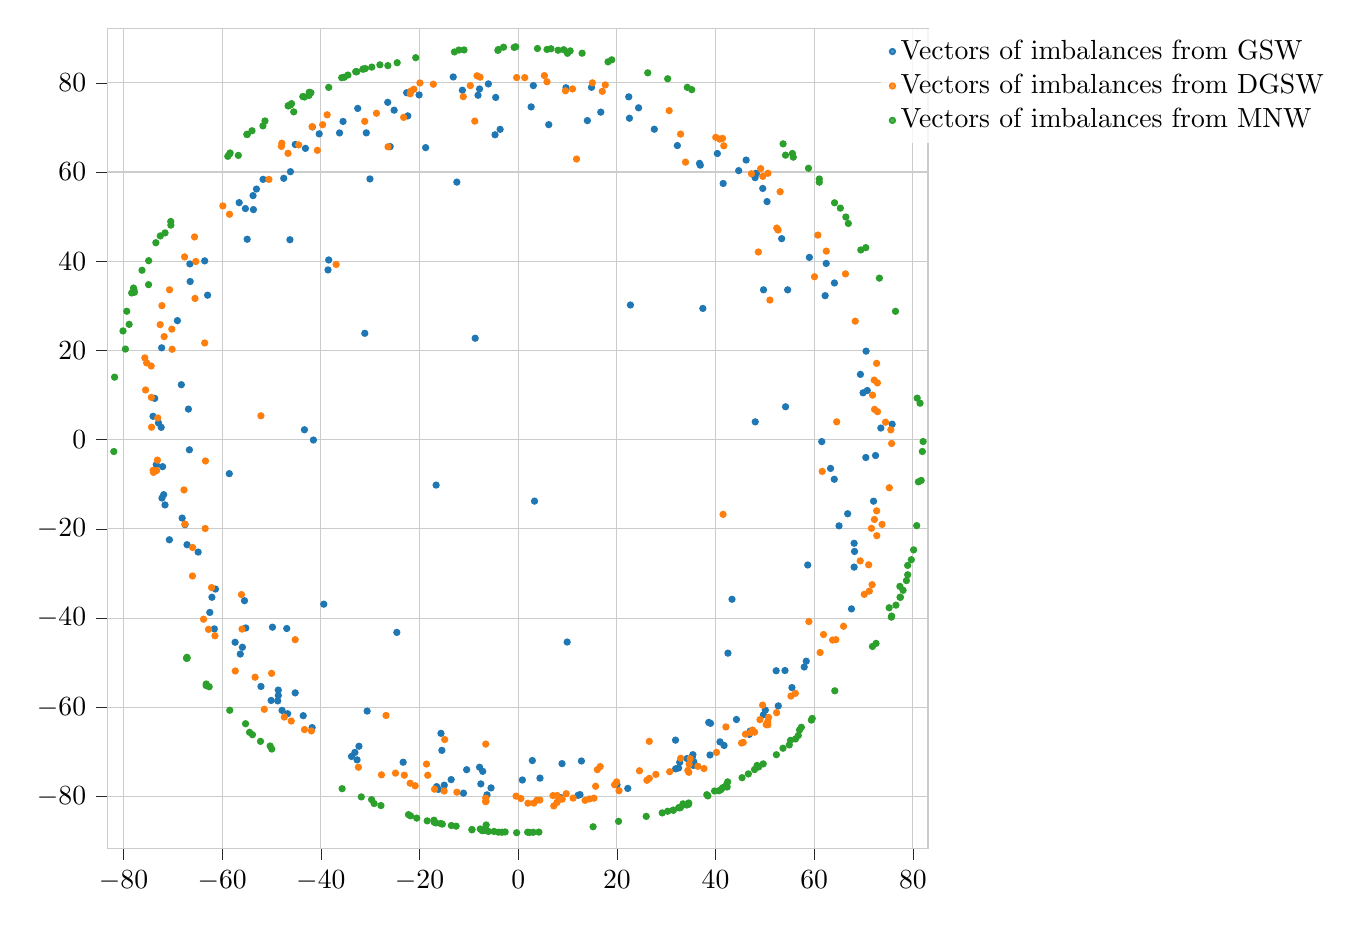
\begin{tikzpicture}

\definecolor{darkorange25512714}{RGB}{255,127,14}
\definecolor{darkslategray38}{RGB}{38,38,38}
\definecolor{forestgreen4416044}{RGB}{44,160,44}
\definecolor{lightgray204}{RGB}{204,204,204}
\definecolor{steelblue31119180}{RGB}{31,119,180}

\begin{axis}[
width=12cm,
height=12cm,
axis line style={lightgray204},
legend cell align={left},
legend style={fill opacity=0.8, draw opacity=1, text opacity=1, at={(1.5,1)}, draw=none},
tick align=outside,
tick pos=left,
x grid style={lightgray204},
xmajorgrids,
xmin=-83.2067624270446, xmax=83.0759530249345,
xtick style={color=darkslategray38},
y grid style={lightgray204},
ymajorgrids,
ymin=-91.6880388118292, ymax=92.2485111427919,
ytick style={color=darkslategray38}
]
\addplot [semithick, steelblue31119180, mark=*, mark size=1, mark options={solid}, only marks]
table {%
32.2584044214495 65.9386568763999
-30.78512025231 68.7889702577337
72.440364565148 -3.56084714298024
-31.08992823135 23.8444022021331
35.5940580599794 -72.2128724567416
58.3909025477593 -49.6674823565428
-72.2037407846078 -13.0958189620082
35.271918282449 -71.2297903844228
-70.699012578559 -22.4460881260352
70.4652216125932 -4.00381322735277
27.5934943162783 69.6029860657221
65.0417469823307 -19.3261587504926
-25.9445743564324 65.7012602015526
38.8841863228764 -70.6977027995228
40.9061831319462 -67.7646673711337
-22.3711169617507 72.5916881875057
-36.2085163933464 68.7732186441355
49.728609698667 33.5941692901107
-49.8110189841752 -42.0433348741018
-32.6558874754734 -71.7918919654906
47.0140395044545 -65.376244693136
-48.6278373077012 -56.1488603780263
70.5220708892224 19.8447876360503
62.4324183640879 39.5100054387699
-46.1585774720407 60.0802314476599
-35.496671284056 71.3509297553594
-43.3250343072014 2.2214075663531
-72.0750252369792 -6.05379458738223
73.5145546414646 2.60061960733761
-15.469635509439 -69.6645520046981
9.92858201556728 -45.3851226072271
-63.5445210013635 40.0852154036615
-51.7117306687373 58.3650565517191
36.7663576635539 61.9446932226637
-8.71521495511577 22.7409185309617
12.1435678304721 -79.7450793566272
-47.8620432214491 -60.7007404143714
40.3750347243597 64.1489314096843
22.4120058248491 76.8646097792012
-25.1440952192131 73.8696031640521
-55.4774723063401 -36.1100611532003
2.62989521214063 74.6121468237154
8.61722999023134 -80.2553914236107
55.4878494652078 -55.5903127999807
-48.6184819841757 -57.3612228608793
36.9147915241226 61.5437715069629
69.914509949494 10.5052875141256
-11.0951599426725 -79.2565652483544
-30.6156024475913 -60.8565302832617
-3.65711718638823 69.5746674390981
63.3174984774895 -6.44555860704591
46.8469333120392 -66.0782918849572
-64.8718044398264 -25.2050458936034
-7.56833618037572 -77.1839710466772
-11.310144915538 78.3473852607746
2.86904121527245 -71.9475349778482
44.695510910438 60.3186013876898
-5.50170588316871 -78.0793195171212
38.6270224756657 -63.3976570441669
75.8031921042529 3.47176771140928
48.0122511931596 58.7478276418118
-4.55826082244179 76.7306598611441
-41.7650338403545 -64.5622905627959
53.409505893534 45.0695346414368
8.88526307026061 -72.6352984043277
-20.0842436314704 77.2946278674008
-48.739557861863 -58.5738919061177
32.5151997855299 -73.6164900702865
12.5336161467112 -79.5892218207455
35.4973356973301 -73.0328014368945
70.7624473395153 11.011416410362
-32.5252717803079 74.2671002390158
-10.4439644224755 -73.998403668327
42.5154700631192 -47.8691247971493
-72.3580516470113 2.76556191728851
41.7334131515087 -68.567040369269
48.050722427563 3.98964067231821
-6.31927292208101 -79.6413727229891
-15.6454859827255 -65.8530219467586
-52.1432394645244 -55.3362868941948
-45.192408960536 66.1849226604328
38.985906930474 -63.6023002403114
-4.69326586973153 68.3523235645167
-55.8997307746974 -46.5433773211604
0.849514366543625 -76.3065008907066
-43.1223552834311 65.3090909826903
-41.7044837624707 70.1181020124392
-74.0158614631308 5.23490266644007
-62.5066619900689 -38.7359985560885
54.197108459558 7.37808465362673
-46.7378168904591 -61.4502786377574
22.2169490391029 -78.1998468213536
67.5611563618523 -37.9437325271889
-7.19194964254755 -74.3726480542728
22.7472306020448 30.1917922504671
68.1846601544919 -25.0638648796997
52.7224603006108 -59.6915580335686
-68.1124833311236 -17.5880196284312
-43.5691012360639 -61.8882003531607
9.68721978321953 78.9026185806715
-62.9540297572674 32.3913549035316
-18.7579787045758 65.4731834425465
20.0302413676354 -77.3671964590653
-13.5855615281493 -76.2214345403727
-69.0742244525684 26.6786143688733
72.0355762419608 -13.7972661302186
-67.5327509300474 -19.0522783873151
-67.1228588819719 -23.5548738064781
-72.9097524679152 3.74287434954817
54.080836277382 -51.7656746726365
69.3668765576836 14.6401594995066
31.9109145158549 -73.8055932753755
54.6218699951625 33.5876366060071
-66.5475315302179 39.40241566771
-68.2761609648053 12.3206924436541
46.2087389936537 62.6854993502268
-66.6428013339522 -2.27611578225907
-57.3759483342749 -45.4321256438847
-47.5172505829085 58.5948273066201
66.7824749745596 -16.6132791464255
-38.5449274390525 38.0546890743992
-71.856018355598 -12.3346633205556
57.9791987046803 -50.9732760619459
61.5350210646747 -0.436132777924667
14.8625614729461 79.0007660917453
-46.9069147680345 -42.3445945471387
-16.181506899167 -78.4131605836978
-39.4047183293266 -36.8883186447915
-62.079009196256 -35.339780932805
-71.5854419791736 -14.6332911579964
-66.4897265970382 35.4564581377113
43.342833219258 -35.7828768319551
-55.2145417893679 -42.2223366512621
-30.0494955875644 58.4569744082907
37.4307325804791 29.4240644199051
-50.0741891133751 -58.473993103024
-6.03830071068439 79.7650747798212
-61.5929339117119 -42.4289545460987
44.2394571824595 -62.7406764068255
-32.2757940906564 -68.7433490573526
-33.7845312277856 -71.0284971743076
-40.3388139928347 68.5642946329428
-72.266582565546 20.5873199674641
-24.5996313535525 -43.2132058432298
-53.0483658673079 56.1874880605418
-14.9821509577675 -77.4682263504023
-58.5565973661462 -7.62276512830875
-66.8389041330287 6.84797938972953
-53.7402545616911 54.7164641076597
-12.4310245384575 57.7434513326038
59.0236570301686 40.8685240561386
50.4446223153189 53.3717984306408
64.099527024871 35.1318418690043
32.7374547673931 -72.3486684735372
3.07510827014208 79.3839490435443
-38.4040307836502 40.2958250145425
-7.83144186364703 78.6300382649299
68.0977007456207 -28.5755211810739
-16.6345637408787 -10.1854716518513
-45.1918547473977 -56.7716551550004
41.5503266464487 57.4350214709958
-61.3567253156031 -33.5013565774428
-41.5033709419344 -0.0849629376979833
35.409695865696 -70.6359754758922
-73.3507634709704 -5.61283228700009
-22.6064612865655 77.7813672044065
31.8966863787351 -67.3724136792563
34.2348354086764 -71.5002136331364
-23.3164788052521 -72.3204791578254
-26.4413144487601 75.6303237862724
14.0247810391753 71.5282771805199
-56.321515260361 -48.0711905268262
62.2225109291443 32.282114560062
52.2926033363182 -51.8150547801773
22.5496147940758 72.0678489342606
-73.6724980883283 9.25582439480754
48.1573099067193 59.7074167018134
50.1005687885256 -60.6353015981225
-46.2663411121317 44.8260452768995
-33.1019141188891 -70.1294637966069
64.0696569961187 -8.87697285071274
-56.5544016901305 53.1436754311971
4.42072127242031 -75.8910310450107
6.19905164153228 70.6269514729997
12.8205115143945 -72.0479931370027
-54.9299979002684 44.9322889061776
49.7056294095111 -61.7056591199924
48.2690935077609 59.6216466570029
-53.6659914487213 51.5796887851568
68.0945920174679 -23.2365582192899
58.6941984750679 -28.1026220069943
-13.1658805954465 81.3210953821928
24.4031648247729 74.3980975889671
-7.82856271221485 -73.4499372459839
3.30903221905349 -13.7852308677481
-16.5266150568404 -77.7979469097883
49.5721093210683 56.3229302952462
-8.13971878634583 77.2139458229984
-55.2909405253252 51.81794402212
16.7432820345378 73.4320509897254
};
\addlegendentry{Vectors of imbalances from GSW}
\addplot [semithick, darkorange25512714, mark=*, mark size=1, mark options={solid}, only marks]
table {%
-6.57300003808273 -68.2611608711121
5.31328927030602 81.6283790119687
-71.764354904977 23.1061308959195
-63.4449039640438 -19.9195951796147
-8.33970209706928 81.5810856990458
-47.9101807910426 66.4691109134433
1.3306360425668 81.171353822595
-62.7735894322806 -42.5364377764579
71.8291420588586 9.98139317644557
61.8898869585487 -43.6865105784712
7.21249723903866 -82.1247637677807
-74.3139818836647 2.79455174815397
-43.3152096732541 -64.9996963741004
75.2276854501355 -10.788391977236
32.9430261449679 -71.4351538792013
19.9517494799329 -76.7281064038012
-47.9979711370703 65.7603383176248
-7.72375358766734 81.2740390108251
-27.711188472057 -75.1495909527575
37.6566222252295 -73.7475013040384
-8.7926184027841 71.4189889184638
72.6955594175556 -21.5271654002011
47.2875546074722 59.617621077416
55.2841557319299 -57.4939438779893
-6.58274032496308 -80.3523689128115
60.7456873960461 45.8617901759081
-75.3165197324567 17.216718113501
-18.5803366136032 -72.7391971670199
-0.421043077751697 -79.9280589745303
-66.0297306902367 -30.5649825808335
72.2345366146534 6.78542359343683
-46.6530675422628 64.1996535494944
60.0634914188462 36.5307859395959
19.5424999298566 -77.3764118273183
30.7078119049722 -74.4468398775456
-63.3884134781183 -4.78155107552455
-52.1459194382976 5.34354297225723
-23.216902282054 72.2580407139287
26.5830481933362 -75.948582008923
64.3969827182105 -44.8482920275507
-28.7210397037759 73.1849081553127
36.4188304027162 -73.242099852905
53.1012894746923 55.5846322390891
9.72805718275821 -79.3823517150815
-40.699251040215 64.8690873864756
46.0770794592862 -66.028882310976
-56.0920735781599 -34.7379747341882
61.6191123852367 -7.11831705077342
72.2076271283572 -17.8935594097667
41.4205859686657 67.5415040179798
-46.0015056181685 -63.0884053114322
17.6619460169287 79.5375825835704
61.2038532603695 -47.7256693729759
50.2753507789513 -63.8940979001035
-63.7760764439446 -40.2584247845739
-51.4678548928031 -60.4561968279941
-73.3006340439803 -6.94216649237462
58.9250225111237 -40.7823741948326
-47.4051195235264 -62.1922959576463
11.8346180209683 62.9157280884327
-74.3533279637824 9.46918678085542
49.0058957476429 -62.7863491657238
-72.569583688022 25.7897082977302
-14.8964229973282 -67.2335424915798
-36.898273563601 39.2833113486128
-75.5233101730811 11.1433872340756
66.3379821833856 37.1733967869614
75.6961200902037 -0.855663772490673
-41.9195823451489 -65.3026016396553
-0.313063649434285 81.1890994125047
52.3827214982965 -61.2169024394471
-58.5106022455496 50.5310991902242
-17.1980055153357 79.6901844251516
74.4626558925317 3.90962509646072
-21.7366262033914 78.1685181778511
34.3881107362911 -74.1794393887005
-59.8567668074318 52.4035276098963
51.021635059922 31.2934497951315
-72.2105258327193 30.0434719454017
-73.9947183137871 -6.87707390302968
50.5833362841406 -63.2342888641987
40.8602617010832 67.382366964869
-38.7197732847345 72.8345266265523
-16.954667480472 -78.3699687247616
-73.923973086827 -7.33905734184872
-67.7421788494786 -11.2682498321696
-49.9830050847466 -52.3968606951822
71.1774070923227 -33.9552330960755
-15.0099760098353 -78.7707975887178
65.9468289478493 -41.8467472661402
3.81195050861152 -80.8322200839502
33.9203784737362 62.226702687568
32.9206691667439 68.512121918567
52.4129614814392 47.4314990433144
40.0500943358723 67.7793933447627
-75.6792169406868 18.3315409155097
47.0949450897698 -65.655360511689
-73.1284594732511 -4.58900249557341
-32.3882612426196 -73.4438222093753
-70.2068878964051 24.7797250499416
56.1802781596985 -56.8856664042302
50.7518339126723 -62.2824305654851
-55.9746396122132 -42.4743244734344
-21.887559145259 77.5412237983377
71.7409962597615 -32.5184588161948
42.1092828388692 -64.4087617587658
41.5316446153193 -16.7504781530775
48.6831535137112 42.0716193908679
-26.3749714172762 65.6590299810163
-67.6199481225327 40.9797545425837
15.6988994752527 -77.7137583741195
15.3589943744872 -80.3911288201285
70.1548389217906 -34.6786292149383
72.8366458199767 6.26979190842479
50.6215690734576 59.7221656184365
8.22525679937225 -80.7724163313869
72.8207966405374 12.7269079974426
-21.1434831835054 78.5618381464854
-9.70837918060963 79.3804590860885
-6.60926846617041 -81.1571064837996
24.5893168574033 -74.2429415588415
62.4516183678715 42.2693896922943
20.4422566121218 -78.7043640262414
14.4367007422784 -80.5604606592273
72.6649637606492 -15.9591100495488
34.5841492174828 -74.5763020266891
-63.5462465243349 21.6818421277734
47.4971644940791 -65.1061947166628
27.9107679083036 -75.0578091364408
16.6251976328391 -73.3028640258055
45.2804507776418 -68.01071383502
-41.7655467255293 70.1589189138736
7.85134253805627 -81.3566798147062
-74.3882078494514 16.5159830225486
30.6076420354553 73.7720387278967
45.6169097978524 -67.8922297911005
75.5386169560949 2.19494710819997
-18.3329399939065 -75.2504775398938
52.6816586996245 47.0076687033763
-62.1456745635549 -33.1685952753351
-65.3446064858711 39.9436891474197
16.0414766261006 -73.9862045559487
47.9277978675119 -65.5817819912364
64.5613458536562 3.99092816219679
-65.9956091469268 -24.1757734179857
-39.6343408296442 70.6160439478426
73.7607409974621 -18.9948589641752
71.6136020356969 -19.8846487073678
11.1325222087021 -80.3659572563612
-61.4642427781268 -43.9639579740379
-21.8954907230776 -77.034649851516
26.0911664307507 -76.3752101954848
4.38907194027385 -80.8097514704446
-70.1468409669891 20.2668363372205
-65.5087742368552 31.6658549539105
11.0210635208653 78.6301103204124
-65.5961249796429 45.4535994795794
69.3291910409258 -27.1810131660296
-24.8659481292113 -74.7702004638136
71.041901089032 -28.0609331311978
-45.1973778751478 -44.8466445126558
13.5624378474542 -80.8644813434682
49.5400014350438 -59.5193081179167
40.1998641919371 -70.1229246785335
17.0433444172601 78.0923551620482
-70.6669754806265 33.5997661723637
-44.4978134670329 66.0870028806813
7.05896022958024 -79.8073269067423
-6.51743134451127 -81.0819837991814
-11.1281852549619 76.906086649774
-19.9161240534128 79.9781603061949
3.16276480584934 -81.4822986322097
68.3190041403423 26.5673395410284
34.655935680701 -72.7811297312628
5.8409670183604 80.2398587689081
7.9132141238474 -79.7940079316188
-23.0827154829219 -75.233814862388
1.97867090842553 -81.5034600315662
41.6784704848857 65.8819126647018
-73.0557418654925 4.86799477330016
-57.3441217583035 -51.8583295955288
72.6537922207366 17.1091737642045
15.0352302057771 80.0025909197412
-67.5353241366693 -18.9287325023133
-50.5287383970326 58.348583495255
9.5878300302957 78.218543784947
49.154483598965 60.7613447689411
-20.8765323801118 -77.604648380287
-53.3285637981133 -53.2636074977827
34.8615228034461 -71.5457564737417
-31.1025470949625 71.3638997387965
-26.7835187468224 -61.8410963111955
0.543045751687271 -80.4661432444305
50.6085027768425 -63.9376431718791
72.1715286361006 13.3412486785492
26.5738162950215 -67.6500155330411
-12.4203949680781 -79.0385212378065
49.5892921540261 59.0394212886869
8.9247478527499 -80.58936760015
63.7352328464401 -44.9312747228185
};
\addlegendentry{Vectors of imbalances from DGSW}
\addplot [semithick, forestgreen4416044, mark=*, mark size=1, mark options={solid}, only marks]
table {%
42.2187897858552 -77.3466940442597
78.0231469121335 -33.772395713265
-46.1442669587632 75.0371565746242
69.4476477767307 42.5379254629481
75.1985563375172 -37.6919428587142
-58.3944088406366 64.2769693161983
-7.68638983131354 -87.2883326391492
54.1862309073416 63.7864337255736
-77.7839402022082 33.0503299527512
-12.925007837351 86.9311981623245
-29.6674529170566 83.5328546793324
55.1979254371374 -67.422152465925
65.3080465569369 51.9129513511809
72.5392154462576 -45.6807350341835
-6.48706046095136 -86.3902228239314
-77.9651249025985 33.9935379895219
66.4216824401156 49.9172400231736
-35.7717401312479 81.1592396977042
-3.96406001327461 -88.0084588083677
77.4719971529889 -35.3514852954127
-26.4141920953607 83.8643174162537
48.4301433711403 -73.0356596455354
73.2179300323774 36.2155066766447
-18.44172561986 -85.4690506005778
38.2383618773534 -79.6025673165431
-43.6563871602343 76.9311917968408
12.9579814274716 86.6469198194951
53.6738519633173 -69.1848704004217
-6.86641748124642 -87.6064846195727
-67.1502619090359 -48.8091392879473
25.952205897638 -84.4631909556707
-29.2009909275812 -81.5862073696289
-15.3737235345191 -86.1973798979606
33.415118942956 -81.6568512232002
32.5171405054778 -82.5253907566525
-63.2433479268035 -55.1346343086845
-13.5397525775156 -86.5181613868655
9.99297555677269 86.6187920639674
42.3524908328557 -77.8854860996471
-12.0252739229913 87.3476584597596
18.2103512130162 84.7059395816794
-58.4632973873028 -60.6773029461017
-31.7964522243784 -80.100454634
41.440750669627 -78.0446410923118
78.9541008921074 -30.2920824170314
-0.816888685038943 87.9570067527856
-81.962246186164 -2.66259885460674
48.7456601630974 -73.3852275414089
-54.9535122673688 68.4397524995277
-0.314465846938702 -88.1275241790371
47.9097974854561 -73.9739700930215
-4.89811627385143 -87.8421250721293
29.1934517062559 -83.684335714213
38.4484231358075 -79.8706781766431
59.4310823465951 -62.8796657551419
77.3684818331768 -32.8951184903521
81.6894907532241 -9.14961034195322
-46.6343752078538 74.8300614505986
-73.441099435793 44.155592018068
-42.4045381742229 77.1735003823969
-38.4022279832157 78.9804095118892
-32.9014616767014 82.5024630187932
45.3823545893373 -75.79534019663
-42.015135967352 77.7885277389825
-24.5269357281049 84.511665204645
-17.0038656648721 -85.7987104521118
-67.2212395286512 -49.0403389592042
-29.714228116071 -80.7144225955582
-12.5770188711524 -86.660932938304
-30.9837920304525 83.1987122988655
4.19895235057013 -87.9912690078653
-45.4905720895866 73.4933642416459
-54.9535122673688 68.4397524995277
-31.4424170452379 83.080593053039
-80.0991007782733 24.3774013116847
3.90657479153912 87.6984715536424
9.23359831546317 87.4350928315283
55.5784916184793 64.1616937597938
30.3004919117379 80.9193361225195
-67.0911982352291 -48.9813144653981
-32.9014616767014 82.5024630187932
-54.9535122673688 68.4397524995277
-74.8991285539727 40.1298330980038
42.46385870097 -76.728702545093
78.7022989975578 -31.6002334077482
-31.4424170452379 83.080593053039
-72.5392154462576 45.6807350341835
82.081670601679 -0.424379279241261
-58.8581799496873 63.5287269634791
-4.10727910061256 87.286775600175
10.5310794892521 87.165930242223
-71.5823554952609 46.3548868304919
-22.2351490492534 -84.0696733443516
26.2651293500311 82.2466230933601
58.845015371017 60.8536243618627
80.7813402406485 -19.2799570546429
-50.2725293502983 -68.6895460786956
57.39917924558 -64.4901424303505
-15.7142724725679 -86.0671374615144
-2.96260617632121 87.996348634828
-52.2339566837629 -67.6454324913073
-70.3995840955867 48.1054770938384
49.6661696654906 -72.6974908480675
-28.0291168826783 84.0403418551762
8.08644853861669 87.3085708250168
-21.8257744264935 -84.3408887965517
81.4581303655903 8.17269930820277
-76.2506327791724 37.9768241026871
61.0371406200021 57.7266233929456
20.3463197825398 -85.5787298826736
-35.2624922596778 81.2656100798938
-3.26677630779439 -88.0201786102107
-74.9216103186033 34.7551046023069
53.6997208412113 66.3226738837107
77.4152171453639 -35.329131935907
76.4835647879187 28.7761505072825
-78.3428589370765 32.8968731618872
34.5686869483397 -81.4639775620498
34.5142388198075 -81.7433300218808
-43.3190322947306 76.8342334361762
6.64825965678075 87.6452302822057
-4.00818660309855 87.4801723539888
79.6873211276208 -26.9212330641394
76.5703448041154 -37.1013015513093
32.6999183566784 -82.4965027288624
40.6687172716727 -78.7268494600129
-27.8191683831229 -82.0402572335621
-7.29555819197313 -87.6637845266095
31.4424170452379 -83.080593053039
-9.37443947523563 -87.445908099336
80.8769271823698 9.30640216988008
70.4639975898609 43.0472785477075
-10.9801316187731 87.3793587235945
-35.6893969632735 -78.2513306014348
-79.3390393412207 28.7896107794872
52.3354781922899 -70.6375628327244
41.0949895214153 -78.4695764238237
-46.5302369248153 74.9158533694372
81.1227558728864 -9.45599113924786
-81.8074713904174 14.0147310400486
-51.3311920558631 71.459679452643
-70.4231503194558 48.9129041925724
2.29937861974223 -88.0664238332306
61.0357745160335 58.4421520977969
-63.225046115407 -54.7775440797247
-34.5142388198075 81.7433300218808
-53.9492261309421 69.2618691194463
-42.3524908328557 77.8854860996471
-16.6891348918289 -85.9292208968939
-77.8739093057425 33.5568700747098
-17.080050287812 -85.3224087644127
64.1808437260021 -56.3128138625946
39.795916694841 -78.7730116467664
-53.8606974942242 -66.1543370764642
-20.7739110886551 85.643028796324
18.9631395114811 85.1616663001613
-9.37443947523563 -87.445908099336
-51.7351907591295 70.3541372101725
5.85122805188153 87.4916426484024
-2.64184064075553 -87.9596973653116
-54.4464551680128 -65.6204430482631
46.6577768669396 -74.939248839053
56.2165314509822 -67.1045055940129
-20.5626001914468 -84.8518475173801
34.5142388198075 -81.7433300218808
30.3023194240771 -83.3183047780515
32.6999183566784 -82.4965027288624
-49.944772187605 -69.3668746315776
34.1589629881419 -81.9183726946166
54.9535122673688 -68.4397524995277
59.6023312384644 -62.5014859069912
66.9239989515675 48.4756740505335
-56.7250914543114 63.7318291442794
35.1853402117036 78.4735300110768
64.128029922626 53.1064712474145
-45.9435368464641 75.3453762712079
34.2813998247644 78.9928361589285
-6.66694287554573 -87.5876813976652
-55.2606922057658 -63.6904883792454
56.7833188335 -66.3200011365378
75.6363254119942 -39.7897714255417
3.04039358458121 -88.0311217021388
1.91998541247223 -88.0074535417625
15.1858334477982 -86.7936129072831
-0.488524847611382 88.0884000921092
80.1568253342377 -24.7185706093779
-78.859250043601 25.8521209307207
-62.6325630587417 -55.4056754966273
78.9419470733631 -28.2006883099576
71.806409466616 -46.3726100483838
31.4424170452379 -83.080593053039
-6.02425807777213 -87.8481312656348
-58.4753203369045 64.0726217004867
55.7586695741879 63.3430049946929
57.0319682031286 -65.090020035929
32.9014616767014 -82.5024630187932
81.9266774423736 -2.65104999273622
75.6994830200278 -39.5559136848349
-32.6999183566784 82.4965027288624
-79.614193821701 20.3088491574854
};
\addlegendentry{Vectors of imbalances from MNW}
\end{axis}

\end{tikzpicture}

\caption{Output sums using the modified GSW and DGSW}
\end{figure}

The outputs are shown in the figure \ref{}. We can see that this modification seems like it now minimizes output balance instead of maximizing it, which was surprising to me at least. This seems like it could be useful to sample from unbalanced group assignments, or to find a subset to remove to maximize something. This might be equivalent to an already known algorithm, but if not I think there are probably interesting applications of this.

\subsection{Are vectors with smaller dimensionality colored at the same moment as vectors with more dimensions ?}
We want to know if vectors with a lot of 0's can be found among vectors that are less sparse, as that could be very interesting to solve various problems such as the planted clique.

\subsubsection{Experiment}

\subsubsection{Results}

%\subsection{Can we make the algorithm faster with some clever factorization ?}
\newpage
%\appendix
%\section{This is an appendix}


\newpage
\nocite{*}
\bibliography{references}
\bibliographystyle{plain}

% Add the References to the table of contents.
\addcontentsline{toc}{section}{References}

\end{document}
